\section{Circuito 2}
\label{chap:circuito_2}

Se muestra en la Figura \ref{plot:circuito_2} el circuito sobre el que se trabajará, que constituye un filtro elimina banda o notch de segundo orden. Los valores de los componentes son:

\begin{itemize}
  \item $R_1: \SI{100}{\kilo\ohm}$
  \item $C_1: \SI{3.18}{\micro\farad}$
  \item $L_1: \SI{31.83}{\milli\henry}$
\end{itemize}

\begin{figure}[H]
  \centering
  \begin{tikzpicture}[transform shape]
	% Paths, nodes and wires:
	\draw (-2, 1) to[sinusoidal voltage source, l={$V_{in}$}] (-2, -1);
	\draw (-0.75, 2) to[american resistor, l={$R_1$}] (1, 2);
	\draw (2, -0) to[american inductor, l={$L_1$}] (2, -2);
	\draw (2, 2) to[capacitor, l={$C_1$}] (2, -0);
	\draw (2, 2) -- (1, 2);
	\draw (-0.75, 2) -| (-2, 1);
	\draw (-2, -1) -| (-2, -2) -- (2, -2);
	\node[ground] at (0, -2){};
	\node[circ, xscale=0.1, yscale=0.1](N1) at (2, 2){} node[anchor=west] at (N1.text){$+  \ \ V_{out}$};
\end{tikzpicture}

  \caption{Esquematico del circuito 2.}
  \label{plot:circuito_2}
\end{figure}

\subsection{Analisis y Simulacion}
\label{sec:analisis_circ_2}

Para el analisis se transforma el circuito a su equivalente en laplace como se ve en la Figura \ref{plot:circuito_2_laplace}.

\begin{figure}[H]
  \centering
  \begin{tikzpicture}[transform shape]
	% Paths, nodes and wires:
	\draw (-2, 1) to[sinusoidal voltage source, l={$V_{in}$}] (-2, -1);
	\draw (2, 2) -- (1, 2);
	\draw (-0.75, 2) -| (-2, 1);
	\draw (-2, -1) -| (-2, -2) -- (2, -2);
	\node[ground] at (0, -2){};
	\draw (-0.75, 2) to[generic, l={$\small 100\ k$}] (1, 2);
	\draw (2, 2) to[generic, l={$\frac{1}{3.18\ \mu\ *\ s}$}] (2, -0);
	\draw (2, -0) to[generic, l={$\small 31.83\ m\ *\ s$}] (2, -2);
	\node[circ, xscale=0.1, yscale=0.1](N1) at (2, 2){} node[anchor=south] at (N1.text){$V_{out}$};
	\node[circ, xscale=0.1, yscale=0.1](N2) at (2, -0){} node[anchor=west] at (N2.text){$V_1$};
\end{tikzpicture}
  \caption{Equivalente en laplace del circuito 2.}
  \label{plot:circuito_2_laplace}
\end{figure}

Considerando la salida en circuito abierto, se puede aplicar la formula del divisor de tension sobre la rama formada por la serie del capacitor $C_1$ y el inductor $L_1$:

\begin{equation}
  V_{out}(s) = V_{in}(s) \cdot \frac{Z_{C_1}(s) + Z_{L_1}(s)}{R_1 + Z_{C_1}(s) + Z_{L_1}(s)}
\end{equation}

donde las impedancias de los componentes son $Z_{C_1}(s) = \frac{1}{s C_1}$ y $Z_{L_1}(s) = s L_1$. Sustituyendo y operando algebraicamente, obtenemos la Funcion de Transferencia (FDT):

\begin{equation}
  H(s) = \frac{s^2 L_1 C_1 + 1}{s^2 L_1 C_1 + s R_1 C_1 + 1}
\end{equation}

Dividiendo el numerador y denominador por el producto $L_1 C_1$, se llega a la forma normalizada estandar de un filtro notch:

\begin{equation}
  H(s) = \frac{s^2 + \frac{1}{L_1 C_1}}{s^2 + s \frac{R_1}{L_1} + \frac{1}{L_1 C_1}}
  \label{eq:fdt-circuito-2-simb}
\end{equation}

Reemplazando por los valores especificados de los componentes:
\begin{itemize}
  \item $L_1 C_1 = \num{31.83d-3} \times \num{3.18d-6} \approx \num{1.0122d-7} \text{ s}^2$
  \item $R_1 C_1 = \num{100d3} \times \num{3.18d-6} = \num{0.318} \text{ s}$
  \item $\omega_0^2 = \frac{1}{L_1 C_1} \approx \num{9.88d6} \text{ rad}^2/\text{s}^2$
  \item $\frac{R_1}{L_1} \approx \num{3.14d6} \text{ rad/s}$
\end{itemize}

De esta forma, se llega finalmente a la ecuacion de la FDT vista en \ref{eq:fdt-circuito-2}:

\begin{equation}
  H(s) = \frac{s^2 + \num{9.88d6}}{s^2 + \num{3.14d6} \cdot s + \num{9.88d6}}
  \label{eq:fdt-circuito-2}
\end{equation}

Los polos del sistema son las raices de la ecuacion caracteristica del denominador:

\begin{equation}
  s^2 + \num{3.14d6} \cdot s + \num{9.88d6} = 0
\end{equation}

Debido a que el termino lineal de amortiguamiento ($\num{3.14d6}$) es extremadamente superior al termino cuadratico medio, el discriminante es marcadamente positivo, lo que nos da dos polos reales, negativos y bien diferenciados (sistema fuertemente sobreamortiguado):

\begin{equation}
  p_1 \approx -\frac{1}{R_1 C_1} = -\num{3.14} \text{ rad/s}
\end{equation}
\begin{equation}
  p_2 \approx -\frac{R_1}{L_1} = -\num{3.14d6} \text{ rad/s}
\end{equation}

Se muestran estos polos graficados en el plano complejo en la Figura \ref{img:polos-plano-circuito-2}. Ambos polos se ubican sobre el eje real izquierdo, lo que garantiza la estabilidad del circuito.

\begin{figure}[H]
  \centering
  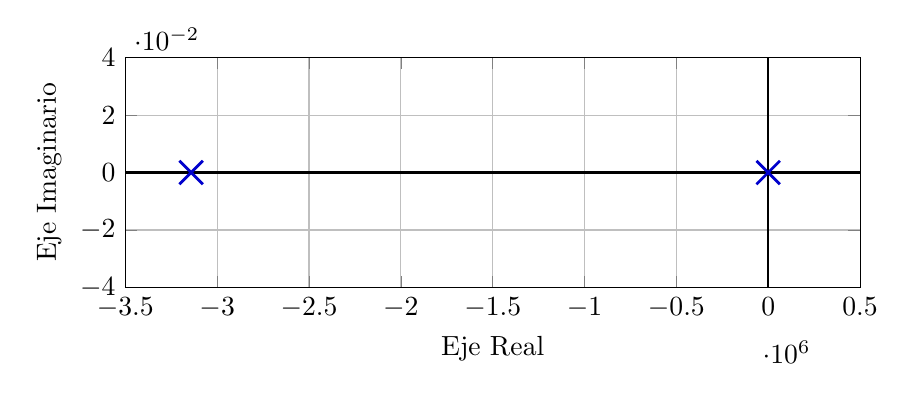
\begin{tikzpicture}
  \begin{axis}[
    width=0.9\columnwidth,
    height=4.5cm,
    xlabel={Eje Real},
    ylabel={Eje Imaginario},
    grid=both,
    xmin=-3500000, xmax=500000,
    ymin=-0.04, ymax=0.04,
  ]
  % Thick x-axis (y=0)
\addplot[
    black,
    line width=0.8pt,
    forget plot
] coordinates {
    (-3500000,0)
    (500000,0)
};

% Thick y-axis (x=0)
\addplot[
    black,
    line width=0.7pt,
    forget plot
] coordinates {
    (0,-0.04)
    (0,0.04)
};

    \addplot[
      scatter,
      only marks,
      mark=x,
      mark size=6pt,
      line width=1pt,
    ]coordinates{
      (-3141690,0)
      (-3.14,0)
    };
  \end{axis}
\end{tikzpicture}

  \caption{Polos en el plano complejo de la FDT del circuito 2.}
  \label{img:polos-plano-circuito-2}
\end{figure}

Se procede ahora a analizar la FDT en el dominio de la frecuencia reemplazando $s = j\omega$, resultando:

\begin{equation}
  H(j\omega) = \frac{1 - \omega^2 L_1 C_1}{1 - \omega^2 L_1 C_1 + j\omega R_1 C_1}
\end{equation}

Para comprobar preliminarmente la validez de la FDT, evaluamos su comportamiento en los extremos de frecuencia:

\begin{align}
  \lim_{\omega \to 0} \frac{1 - \omega^2 L_1 C_1}{1 - \omega^2 L_1 C_1 + j\omega R_1 C_1} &= 1 \\
  \lim_{\omega \to \infty} \frac{1 - \omega^2 L_1 C_1}{1 - \omega^2 L_1 C_1 + j\omega R_1 C_1} &= 1
\end{align}

Esto muestra que las senales de muy baja y muy alta frecuencia pasan sin atenuacion, mientras que a la frecuencia central $\omega_0 = \frac{1}{\sqrt{L_1 C_1}} \approx \num{3143} \text{ rad/s}$ ($f_0 \approx \SI{500}{\hertz}$), la ganancia se anula por completo ($H(j\omega_0) = 0$), confirmando el comportamiento ideal de un filtro notch.

A fin de obtener el diagrama polar de la FDT, separamos la funcion en su parte real e imaginaria multiplicando y dividiendo por el conjugado del denominador:

\begin{align}
  Re(\omega) &= \frac{(1 - \omega^2 L_1 C_1)^2}{(1 - \omega^2 L_1 C_1)^2 + (\omega R_1 C_1)^2} \\
  Img(\omega) &= \frac{-\omega R_1 C_1 (1 - \omega^2 L_1 C_1)}{(1 - \omega^2 L_1 C_1)^2 + (\omega R_1 C_1)^2}
\end{align}

Estas ecuaciones describen geometricamente una circunferencia desplazada en el plano complejo, que cumple con la relacion algebraica:

\begin{equation}
  \left(Re(\omega) - \frac{1}{2}\right)^2 + Img(\omega)^2 = \left(\frac{1}{2}\right)^2
\end{equation}

La Figura \ref{plot:polar_circuito_2} muestra el diagrama polar obtenido de la FDT ideal.

\begin{figure}[H]
  \centering
  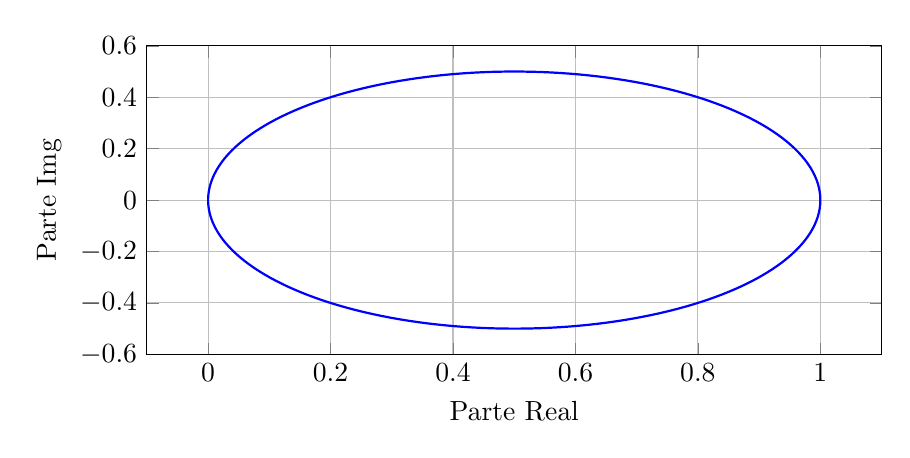
\begin{tikzpicture}
  \begin{axis}[
    width=0.9\columnwidth,
    height=5.5cm,
    xlabel={Parte Real},
    ylabel={Parte Img},
    grid=both,
    xmin=-0.1, xmax=1.1,
    ymin=-0.6, ymax=0.6,
    ytick={-0.6,-0.4,-0.2,0,0.2,0.4,0.6},
    xtick={0,0.2,0.4,0.6,0.8,1.0},
    axis lines=box,
  ]
  \addplot[
      blue,
      thick,
      domain=0:360,
      samples=200,
  ]
  (
      {0.5 + 0.5*cos(x)},
      {0.5*sin(x)}
  );
  \end{axis}
\end{tikzpicture}

  \caption{Diagrama polar de la FDT del circuito 2 (ideal).}
  \label{plot:polar_circuito_2}
\end{figure}

\begin{figure}[H]
  \centering
  \begin{tikzpicture}
\begin{semilogxaxis}[
    xlabel={Frecuencia $\omega$ (rad/s)},
    ylabel={Magnitud (dB)},
    grid=both,
    grid style={line width=.1pt, draw=gray!30},
    major grid style={line width=.2pt, draw=gray!60},
    xmin=1e-1, xmax=1e8,
    ymin=-120, ymax=10,
    width=0.9\columnwidth,
    height=5.5cm,
    legend style={
        at={(0.5, 1.05)}, % x=0.5 (centro horizontal), y=1.05 (por encima del límite superior)
        anchor = south,
        scale = 0.9,
        font=\footnotesize % Reduce el tamaño del texto y los símbolos
    }
]

% Trazado asintótico
\addplot[thick, blue] coordinates {
    (1e-1, 0)
    (3.14, 0)
    (3143, -60)
    (3.14e6, 0)
    (1e8, 0)
};
\addlegendentry{Teórico (Asintótico)}

% Marcador de wp1
\draw[dashed, red, thin] (axis cs:3.14, 0) -- (axis cs:3.14, -60);
\addplot[mark=*, mark size=1.5pt, red, forget plot] coordinates {(3.14, -60)};
\node[anchor=north, font=\scriptsize, text=black] at (axis cs:3.14, -60) {$\omega_{p1} = 3.14$};

% Marcador de w0
\addplot[mark=*, mark size=1.5pt, red, forget plot] coordinates {(3143, -60)};
\node[anchor=south, font=\scriptsize, text=black] at (axis cs:3143, -50) {$\omega_{0} = 3143$};

% Marcador de wp2
\draw[dashed, red, thin] (axis cs:3.14e6, 0) -- (axis cs:3.14e6, -60);
\addplot[mark=*, mark size=1.5pt, red, forget plot] coordinates {(3.14e6, -60)};
\node[anchor=north, font=\scriptsize, text=black] at (axis cs:3.14e6, -60) {$\omega_{p2} = 3.14\text{ M}$};

% Datos de LTSpice
\addplot[thick, dashed, orange] table [
    skip first n=1,
    x expr=\thisrowno{0} * 2 * pi,
    y index=1
] {sim/bode_2.txt};
\addlegendentry{Simulación LTSpice}

\end{semilogxaxis}
\end{tikzpicture}

  \caption{Diagrama de Bode de Magnitud del circuito 2 (Simulado vs Asintótico).}
  \label{plot:bode_mag_circuito_2}
\end{figure}

\begin{figure}[H]
  \centering
  \begin{tikzpicture}
\begin{semilogxaxis}[
    xlabel={Frecuencia $\omega$ (rad/s)},
    ylabel={Fase (grados)},
    grid=both,
    grid style={line width=.1pt, draw=gray!30},
    major grid style={line width=.2pt, draw=gray!60},
    xmin=1e-1, xmax=1e8,
    ymin=-120, ymax=120,
    ytick={-90, 0, 90},
    width=0.9\columnwidth,
    height=5.5cm,
    legend style={
        at={(0.5, 1.05)}, % x=0.5 (centro horizontal), y=1.05 (por encima del límite superior)
        anchor = south,
        scale = 0.9,
        font=\footnotesize % Reduce el tamaño del texto y los símbolos
    }
]

% Trazado asintótico de fase
\addplot[thick, blue] coordinates {
    (1e-1, 0)
    (0.314, 0)
    (31.4, -90)
    (3143, -90)
    (3143, 90)
    (3.14e5, 90)
    (3.14e7, 0)
    (1e8, 0)
};
\addlegendentry{Teórico (Asintótico)}

% Marcas de los polos y ceros
\addplot[mark=|, mark size=3pt, red, forget plot] coordinates {(0.314, 0)};
\node[anchor=south west, font=\small, text=black] at (axis cs:0.314, 0) {$0.1\omega_{p1}$};

\addplot[mark=|, mark size=3pt, red, forget plot] coordinates {(3.14e7, 0)};
\node[anchor=north east, font=\small, text=black] at (axis cs:3.14e7, 0) {$10\omega_{p2}$};

% Datos de LTSpice
\addplot[thick, dashed, orange] table [
    skip first n=1,
    x expr=\thisrowno{0} * 2 * pi,
    y index=2
] {sim/bode_2.txt};
\addlegendentry{Simulación LTSpice}

\end{semilogxaxis}
\end{tikzpicture}

  \caption{Diagrama de Bode de Fase del circuito 2 (Simulado vs Asintótico).}
  \label{plot:bode_phase_circuito_2}
\end{figure}

\subsection{Mediciones de Laboratorio}
\label{sec:mediciones_circ_2}

Para la verificación experimental, se realizó la implementación física del filtro notch utilizando componentes reales cuyos valores medidos fueron:
\begin{itemize}
  \item Resistencia: $R = \SI{100}{\kilo\ohm}$
  \item Inductor: $L = \SI{31.8}{\milli\henry}$
  \item Capacitor: $C = \SI{3.3}{\micro\farad}$
\end{itemize}

El capacitor utilizado en el laboratorio ($C = \SI{3.3}{\micro\farad}$) es muy cercano al valor de diseño teórico de $\SI{3.18}{\micro\farad}$. Con estos componentes reales, la frecuencia angular de resonancia teórica $\omega_0$ y la correspondiente frecuencia de corte $f_0$ son:
\begin{equation}
  \omega_0 = \frac{1}{\sqrt{L \cdot C}} = \frac{1}{\sqrt{\SI{31.8}{\milli\henry} \cdot \SI{3.3}{\micro\farad}}} \approx \SI{3087.96}{\radian\per\second}
\end{equation}
\begin{equation}
  f_0 = \frac{\omega_0}{2\pi} \approx \SI{491.46}{\hertz}
\end{equation}

Los polos del sistema real se ubican teóricamente en:
\begin{align}
  p_1 &\approx -\frac{1}{R \cdot C} = -\SI{3.03}{\radian\per\second} \quad (f_{p1} \approx \SI{0.48}{\hertz}) \\
  p_2 &\approx -\frac{R}{L} = -\SI{3.14}{\mega\radian\per\second} \quad (f_{p2} \approx \SI{500.5}{\kilo\hertz})
\end{align}

Durante el ensayo en el laboratorio, se utilizó un generador de señales para aplicar una tensión senoidal $V_{in}$ a la entrada del filtro. Se midieron las tensiones de entrada y salida con un osciloscopio digital RIGOL. Todas las mediciones de tensión en la Tabla \ref{tab:mediciones_circuito_2} han sido unificadas a valor eficaz ($V_{rms}$) para garantizar la consistencia, realizando la conversión $V_{rms} = V_{pp}/(2\sqrt{2})$ para las frecuencias de \SI{2}{\hertz} y \SI{10}{\hertz} que originalmente se registraron como pico a pico ($V_{pp}$). La atenuación del filtro se expresa directamente como ganancia en decibeles.

\begin{table}[H]
  \centering
  \begin{tabular}{cccc}
    \hline
    \textbf{Frecuencia} & \textbf{Tensión $V_{in}$ ($V_{rms}$)} & \textbf{Tensión $V_{out}$ ($V_{rms}$)} & \textbf{Ganancia [dB]} \\ \hline
    \SI{2}{\hertz}      & \SI{2.40}{\volt}                      & \SI{678.8}{\milli\volt}                 & \SI{-10.98}{\decibel}  \\
    \SI{10}{\hertz}     & \SI{2.62}{\volt}                      & \SI{169.7}{\milli\volt}                 & \SI{-23.76}{\decibel}  \\
    \SI{100}{\hertz}    & \SI{2.5}{\volt}                       & \SI{86}{\milli\volt}                    & \SI{-29.27}{\decibel}  \\
    \SI{1}{\kilo\hertz} & \SI{2.5}{\volt}                       & \SI{90}{\milli\volt}                    & \SI{-28.87}{\decibel}  \\
    \SI{10}{\kilo\hertz}& \SI{2.5}{\volt}                       & \SI{10}{\milli\volt}                    & \SI{-47.96}{\decibel}  \\
    \SI{100}{\kilo\hertz}& \SI{2.5}{\volt}                      & \SI{770}{\milli\volt}                   & \SI{-10.23}{\decibel}  \\
    \SI{200}{\kilo\hertz}& \SI{2.5}{\volt}                      & \SI{1.19}{\volt}                        & \SI{-6.45}{\decibel}   \\ \hline
  \end{tabular}
  \caption{Mediciones experimentales del circuito 2 en el laboratorio (unificadas a valor eficaz).}
  \label{tab:mediciones_circuito_2}
\end{table}

\begin{figure}[H]
  \centering
  \begin{tikzpicture}
\begin{semilogxaxis}[
    title={Comparación de Magnitud del Circuito 2 Real},
    xlabel={Frecuencia $\omega$ (rad/s)},
    ylabel={Magnitud (dB)},
    grid=both,
    grid style={line width=.1pt, draw=gray!30},
    major grid style={line width=.2pt, draw=gray!60},
    xmin=1, xmax=2e6,
    ymin=-80, ymax=5,
    width=0.9\columnwidth,
    height=5.5cm,
    legend style={
        nodes={scale=0.7, transform shape},
        at={(0.05,0.05)},
        anchor=south west
    }
]

% Curva de Simulación de LTSpice con Rser = 50 Ohm y C = 3.3 uF
\addplot[thick, blue] table [
    skip first n=1,
    x expr=\thisrowno{0} * 2 * pi,
    y index=1
] {sim/circuito_2_50omh.txt};
\addlegendentry{Simulación (LTSpice, $R_{ser}=50\,\Omega$)}

% Puntos Medidos en Laboratorio
\addplot[
    only marks,
    mark=*,
    mark size=2.0pt,
    red
] coordinates {
    (12.56637, -10.98)     % 2 Hz
    (62.83185, -23.76)     % 10 Hz
    (628.3185, -29.27)     % 100 Hz
    (6283.185, -28.87)     % 1 kHz
    (62831.85, -47.96)     % 10 kHz
    (628318.53, -10.23)    % 100 kHz
    (1256637.06, -6.45)    % 200 kHz
};
\addlegendentry{Mediciones de Laboratorio}

\end{semilogxaxis}
\end{tikzpicture}

  \caption{Comparación entre la simulación de LTSpice del circuito real (con $C = \SI{3.3}{\micro\farad}$ y $R_{ser} = \SI{50}{\ohm}$ para modelar la pérdida del inductor) y las mediciones obtenidas en el laboratorio.}
  \label{plot:bode_medido_vs_teorico_circuito_2}
\end{figure}

A partir de las mediciones graficadas en la Figura \ref{plot:bode_medido_vs_teorico_circuito_2}, se observa un buen acuerdo general con la respuesta simulada. A frecuencias muy bajas (\SI{2}{\hertz} y \SI{10}{\hertz}) y altas (\SI{100}{\kilo\hertz} y \SI{200}{\kilo\hertz}), los puntos coinciden notablemente con la simulación. En el rango de \SI{100}{\hertz} a \SI{1}{\kilo\hertz}, los valores medidos presentan una meseta en torno a los \SI{-29}{\decibel}, limitados principalmente por el piso de ruido del instrumental, pero registrando el comportamiento atenuador central esperado.

Para registrar con mayor resolución la respuesta en frecuencia completa del filtro en el entorno de la sintonía, se capturó la pantalla del osciloscopio mostrada en la Figura \ref{img:bode_medido_circuito_2}, la cual grafica la respuesta obtenida mediante la Transformada Rápida de Fourier (FFT). El osciloscopio se configuró con una escala de magnitud vertical de \SI{10.0}{\decibel\text{Vrms}/div} y una escala de frecuencia horizontal de \SI{250.0}{\hertz/div}. Con el inicio del barrido en corriente continua, la fosa del notch se ubicó exactamente a dos divisiones del origen de frecuencias, lo cual corresponde a una frecuencia de sintonía de sintonía de $2 \times \SI{250}{\hertz/div} = \SI{500}{\hertz}$, en excelente concordancia con la frecuencia de resonancia teórica calculada de $\SI{491.46}{\hertz}$. Utilizando los cursores del osciloscopio, se midió un nivel de referencia en la banda de paso de $CurA = \SI{-43.6}{\decibel}$ y el punto mínimo del notch en $CurB = \SI{-74.8}{\decibel}$, registrando una profundidad de notch de $\SI{31.2}{\decibel}$. Este comportamiento práctico valida satisfactoriamente el análisis teórico propuesto para este filtro.

\begin{figure}[H]
  \centering
  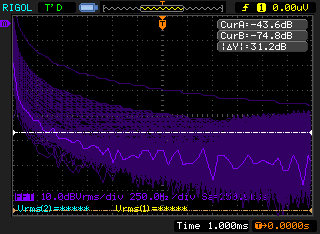
\includegraphics[width=0.8\columnwidth]{images/bd2.png}
  \caption{Respuesta en frecuencia (FFT) del circuito notch real medida en el laboratorio.}
  \label{img:bode_medido_circuito_2}
\end{figure}
